\section{Feature-Space Visualisation}
\label{sec:feature-visualisation}

\begin{figure}[H]
\centering
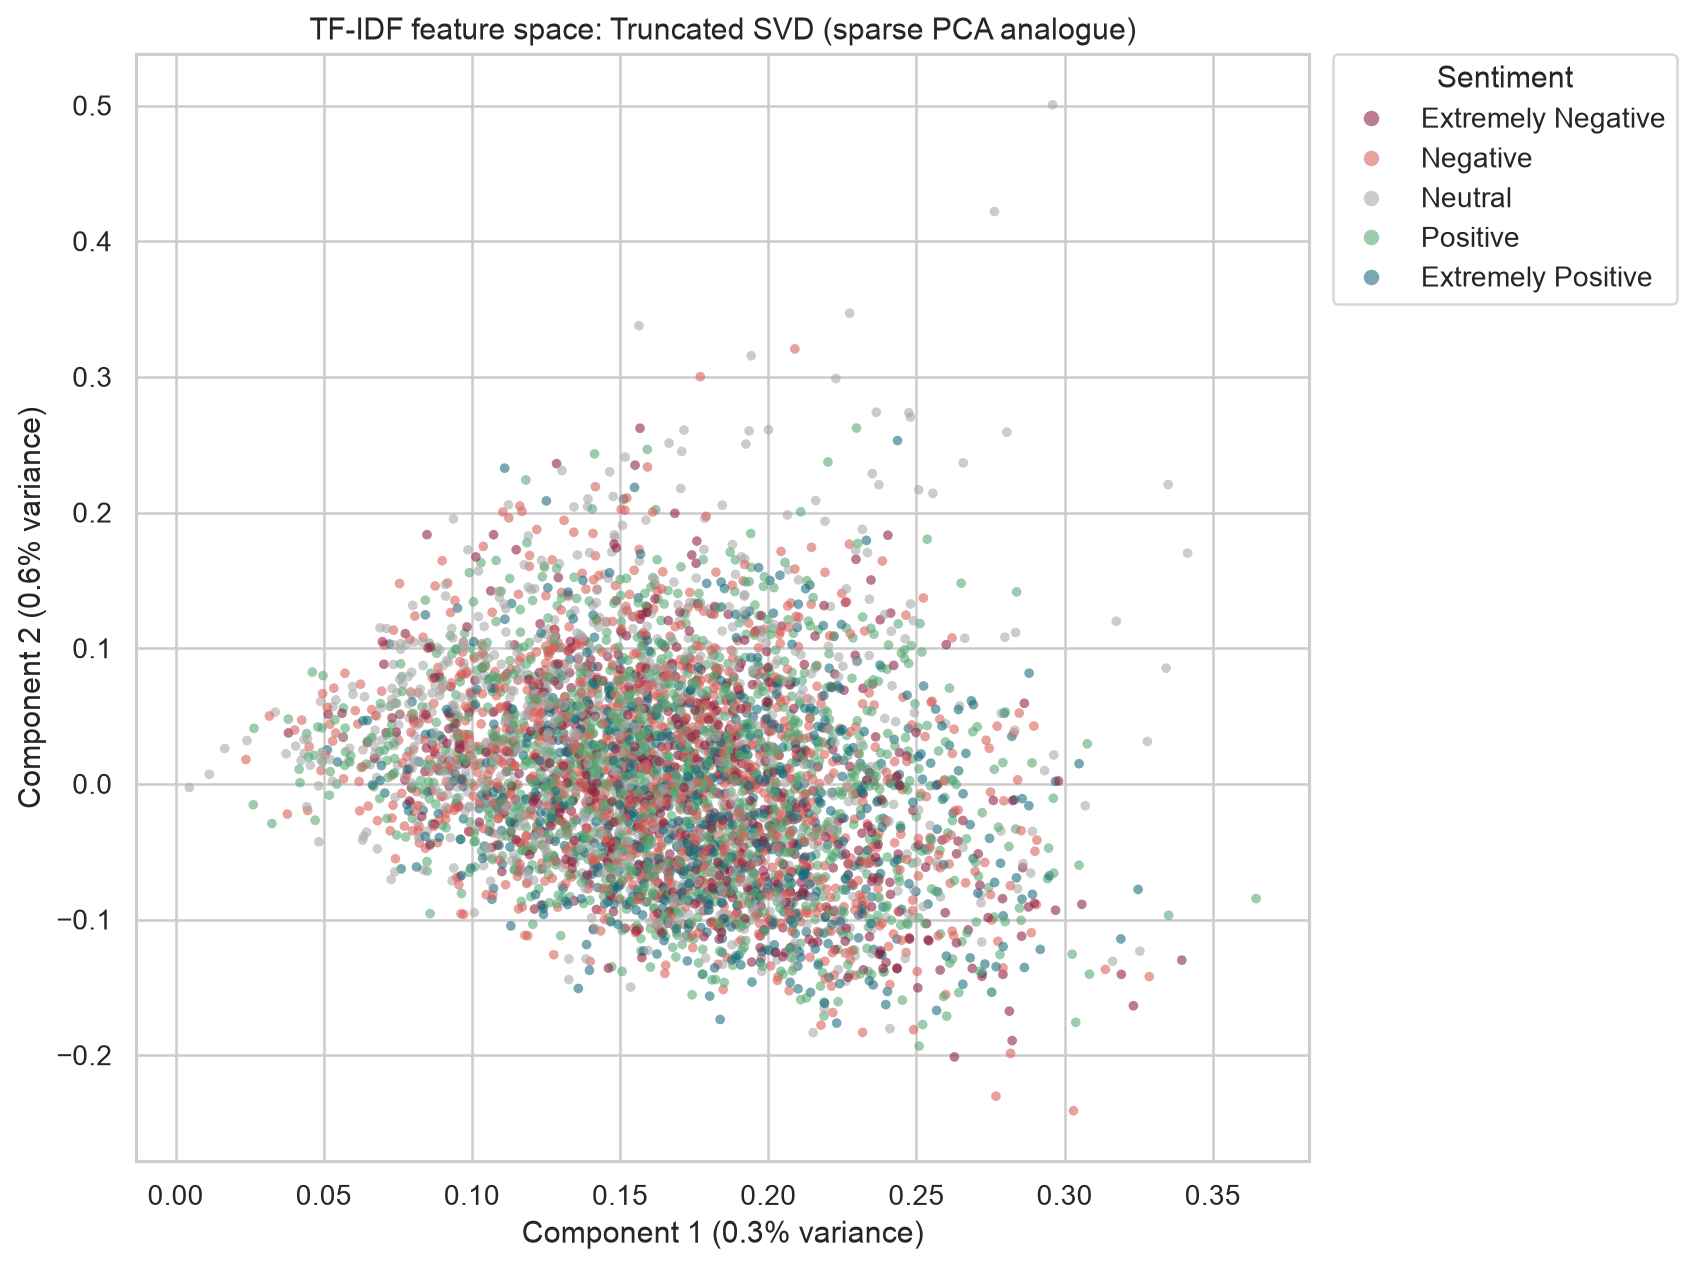
\includegraphics[width=0.49\textwidth]{../outputs/graphics/feature_space/tfidf/pca.png}
\hfill
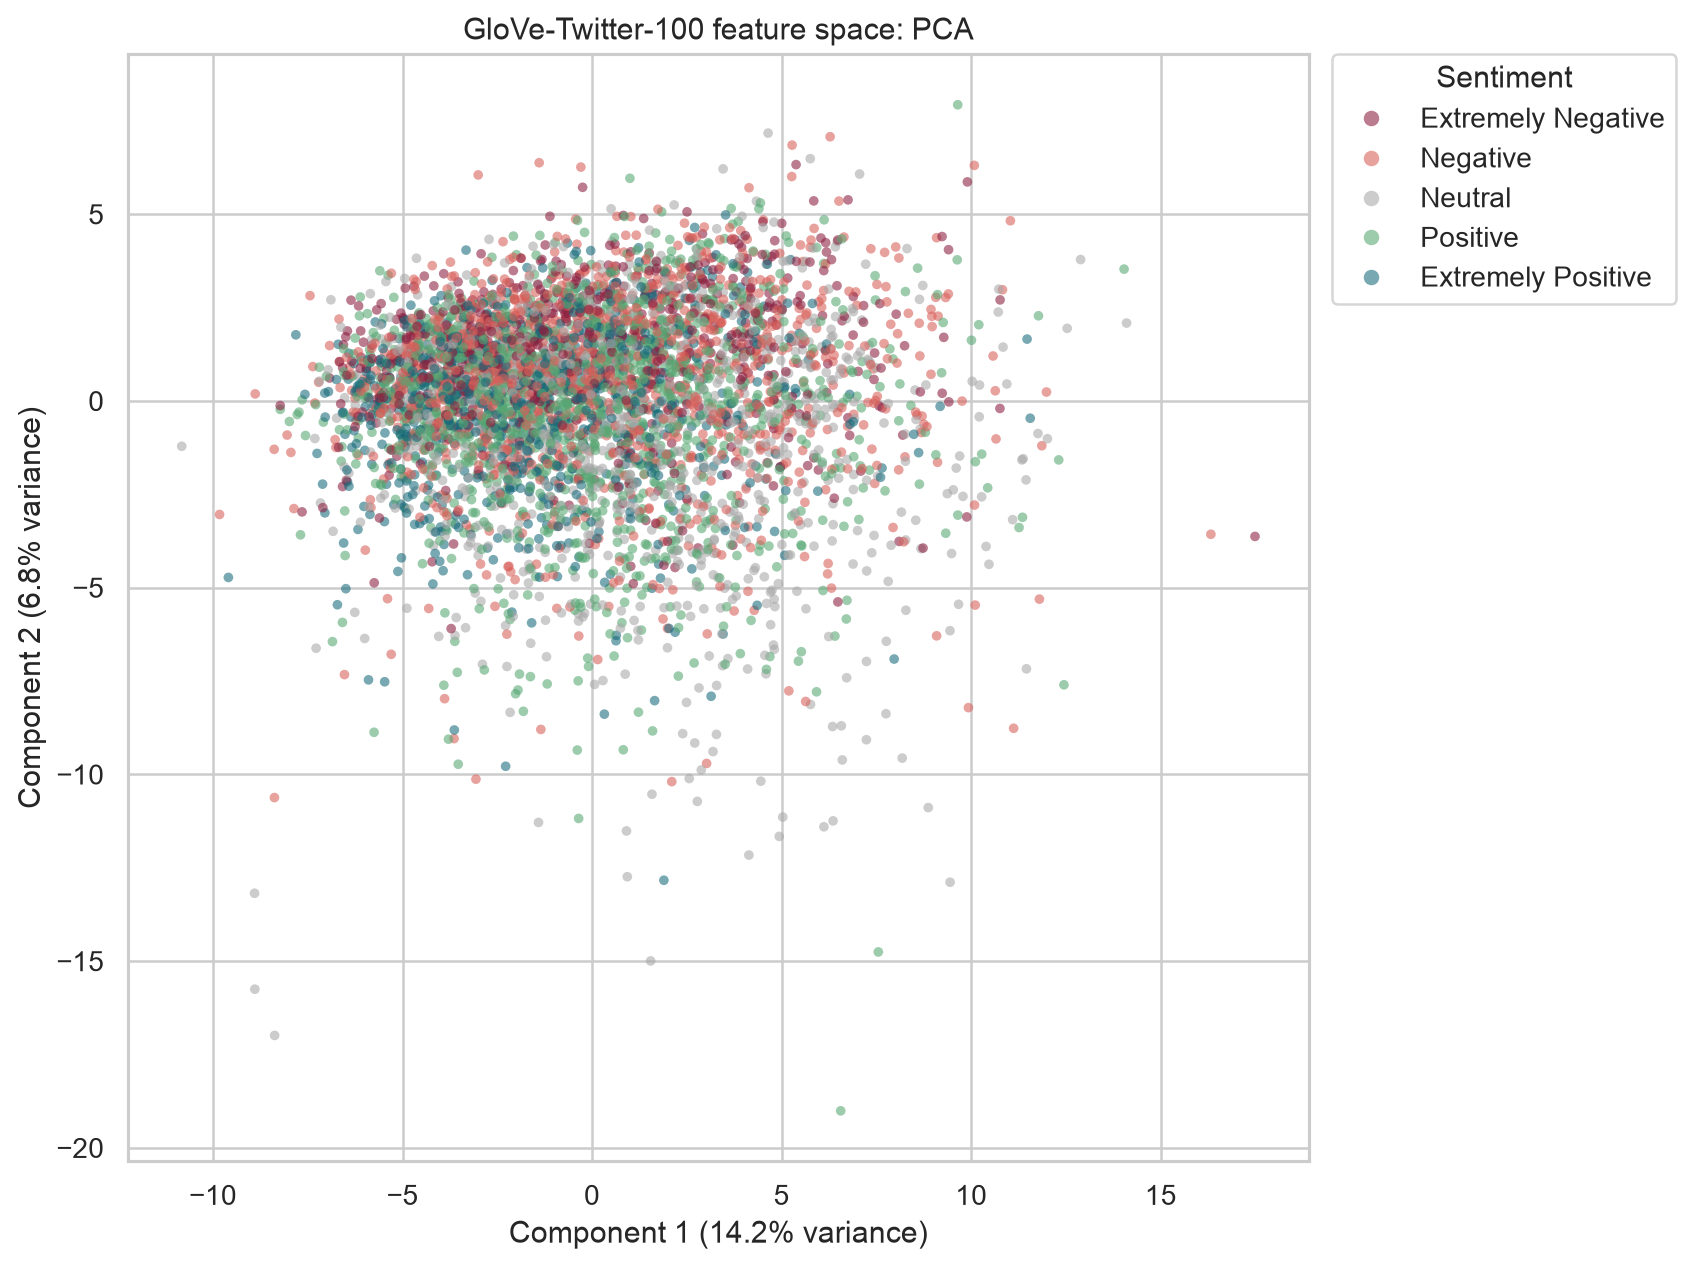
\includegraphics[width=0.49\textwidth]{../outputs/graphics/feature_space/glove/pca.png}
\caption{Linear two-dimensional projections of TF-IDF using Truncated SVD (left) and standardized GloVe using PCA (right).}
\label{fig:feature-pca}
\end{figure}

\begin{figure}[H]
\centering
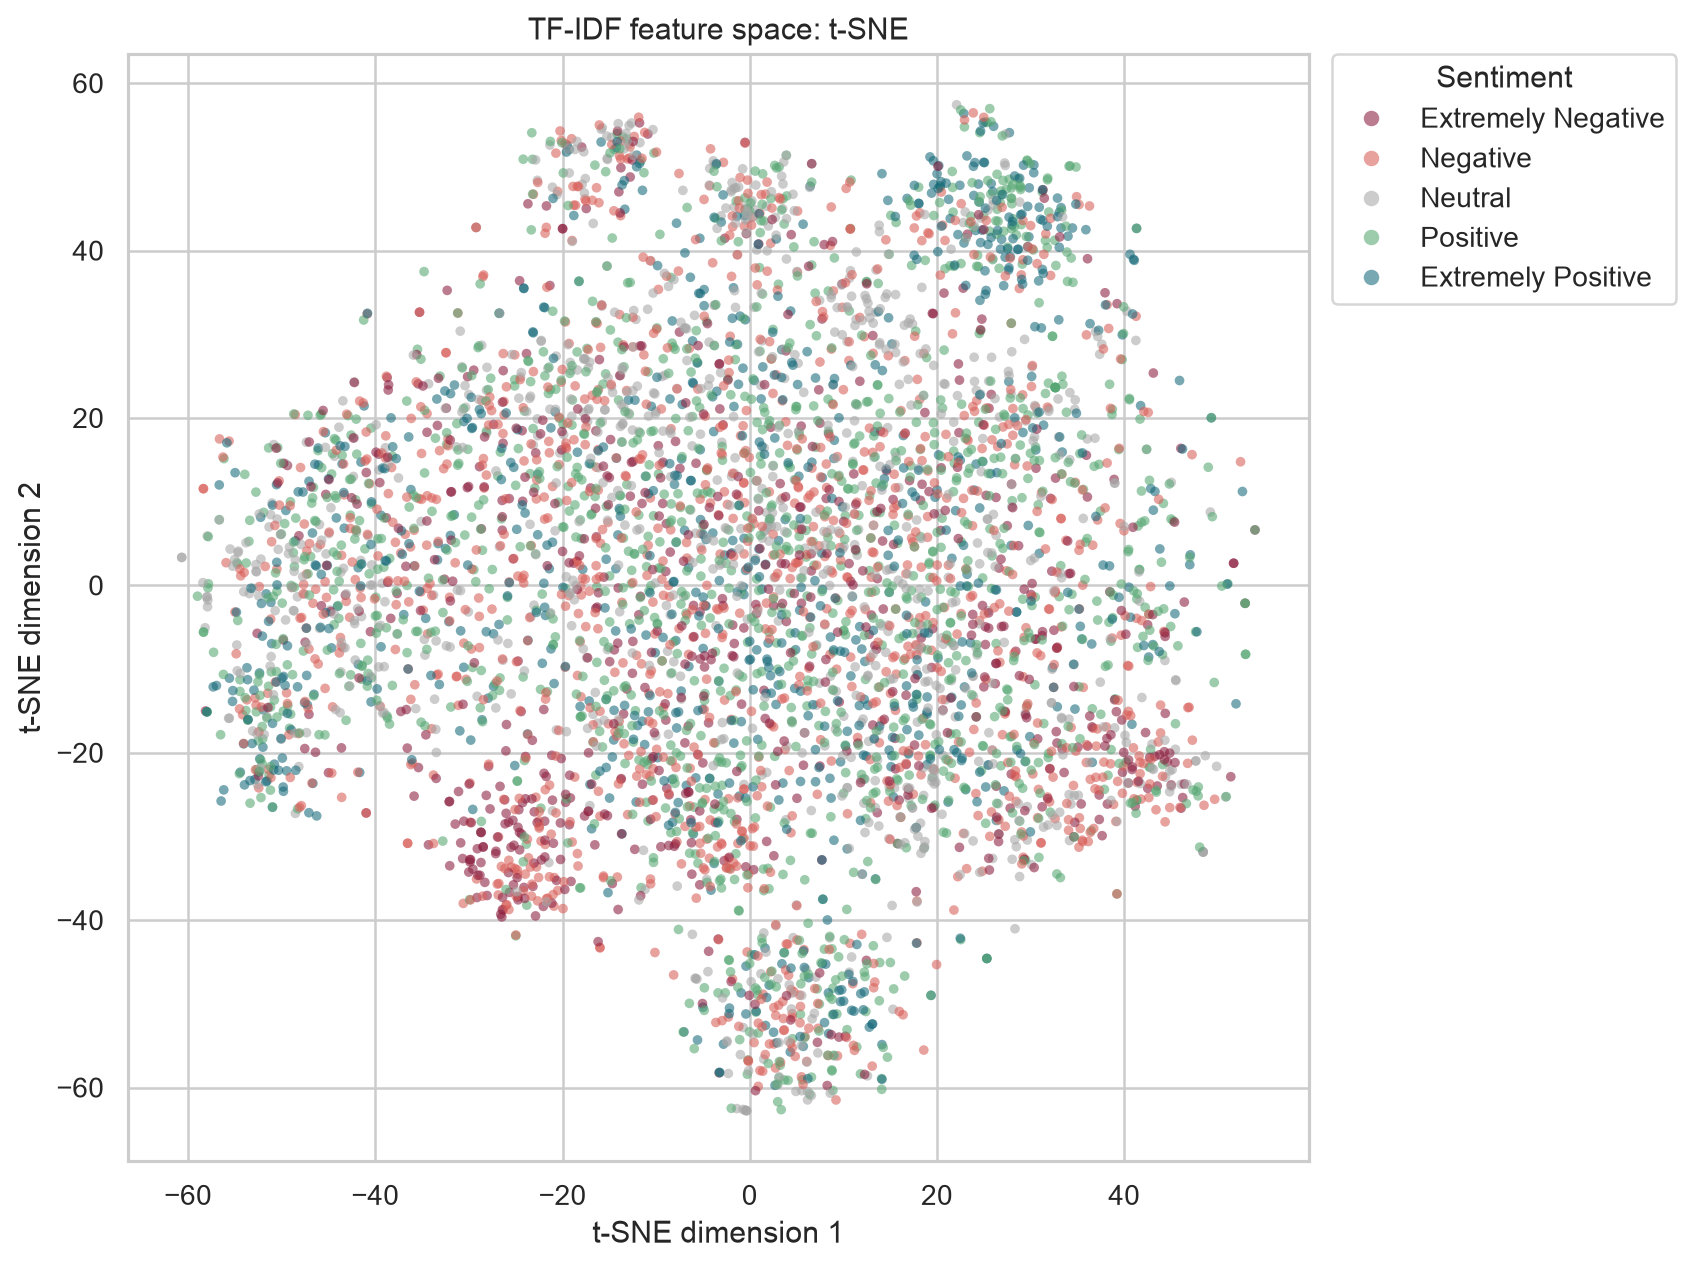
\includegraphics[width=0.49\textwidth]{../outputs/graphics/feature_space/tfidf/tsne.png}
\hfill
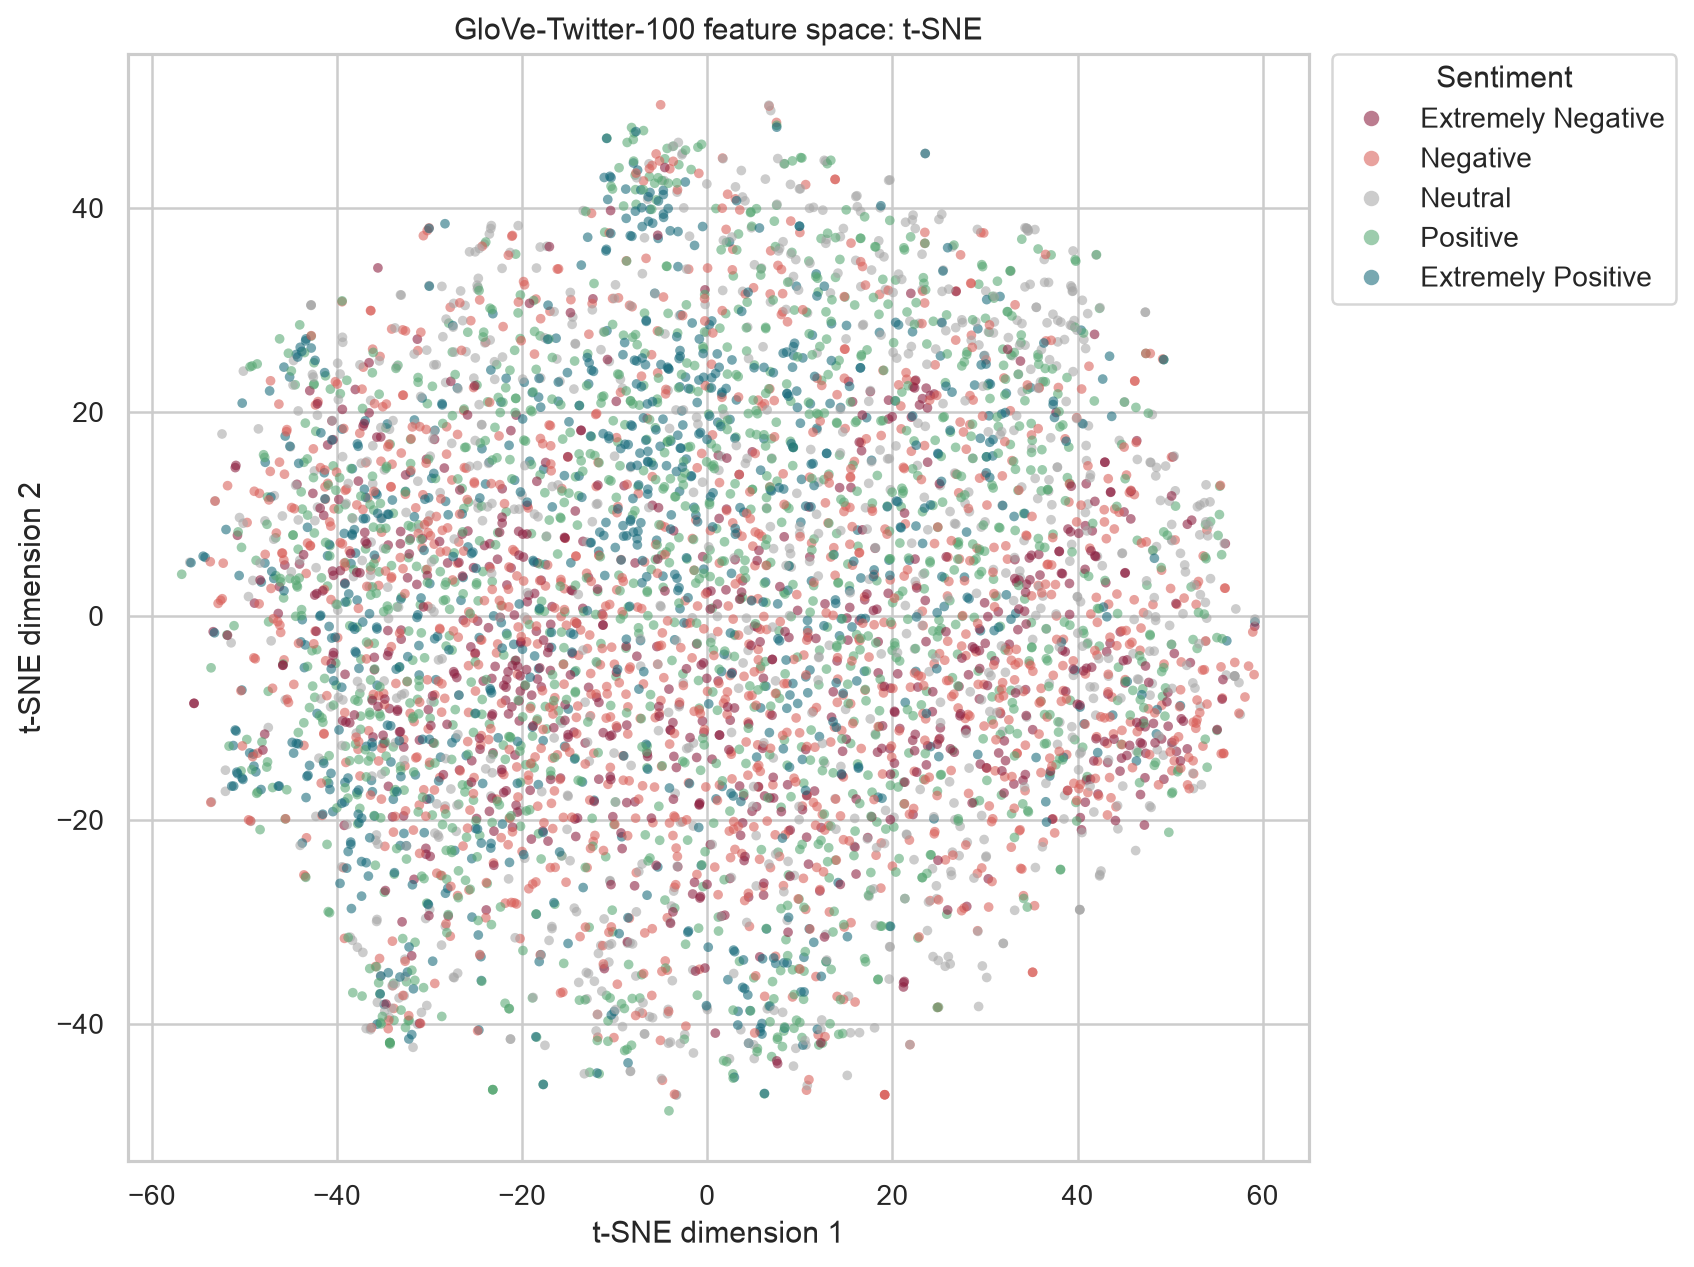
\includegraphics[width=0.49\textwidth]{../outputs/graphics/feature_space/glove/tsne.png}
\caption{t-SNE projections of TF-IDF (left) and GloVe (right), computed from their respective 50-dimensional PCA/SVD representations.}
\label{fig:feature-tsne}
\end{figure}

\begin{figure}[H]
\centering
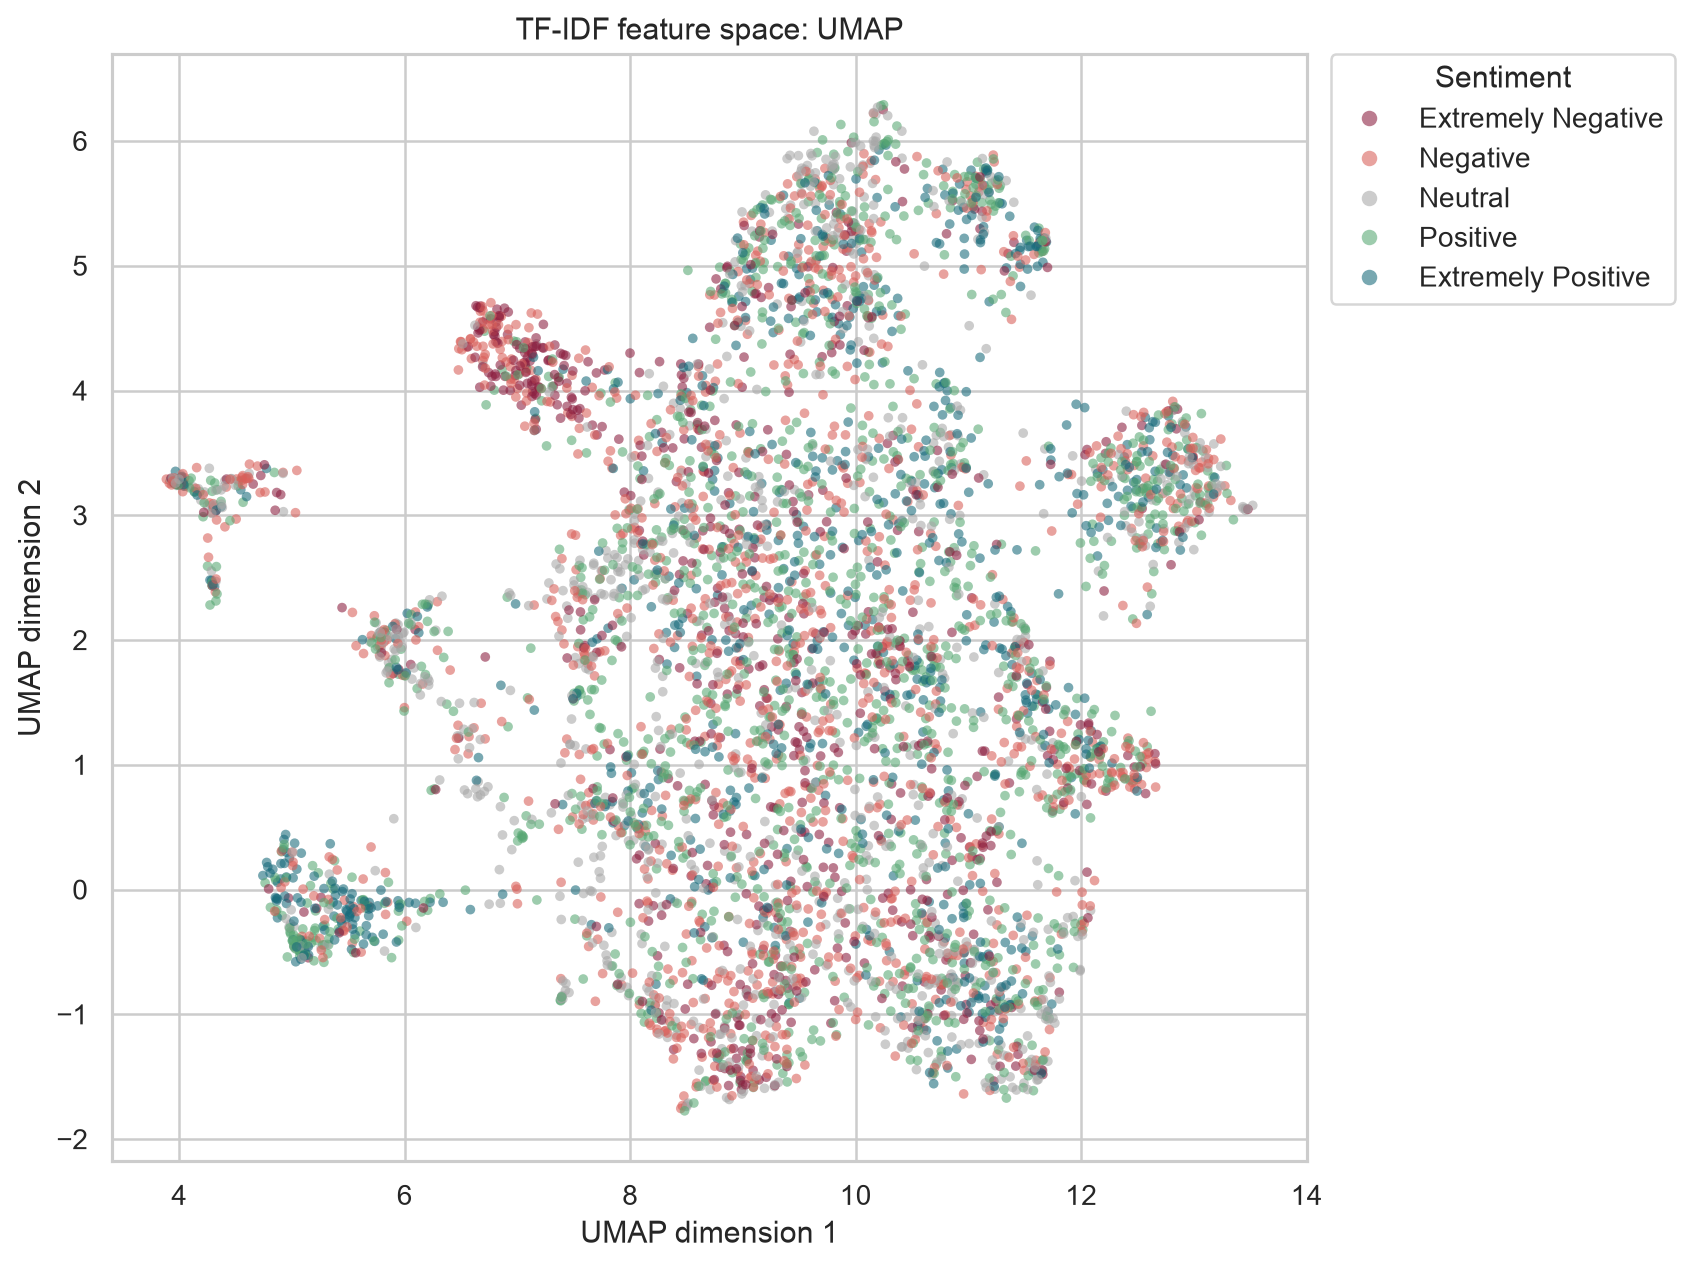
\includegraphics[width=0.49\textwidth]{../outputs/graphics/feature_space/tfidf/umap.png}
\hfill
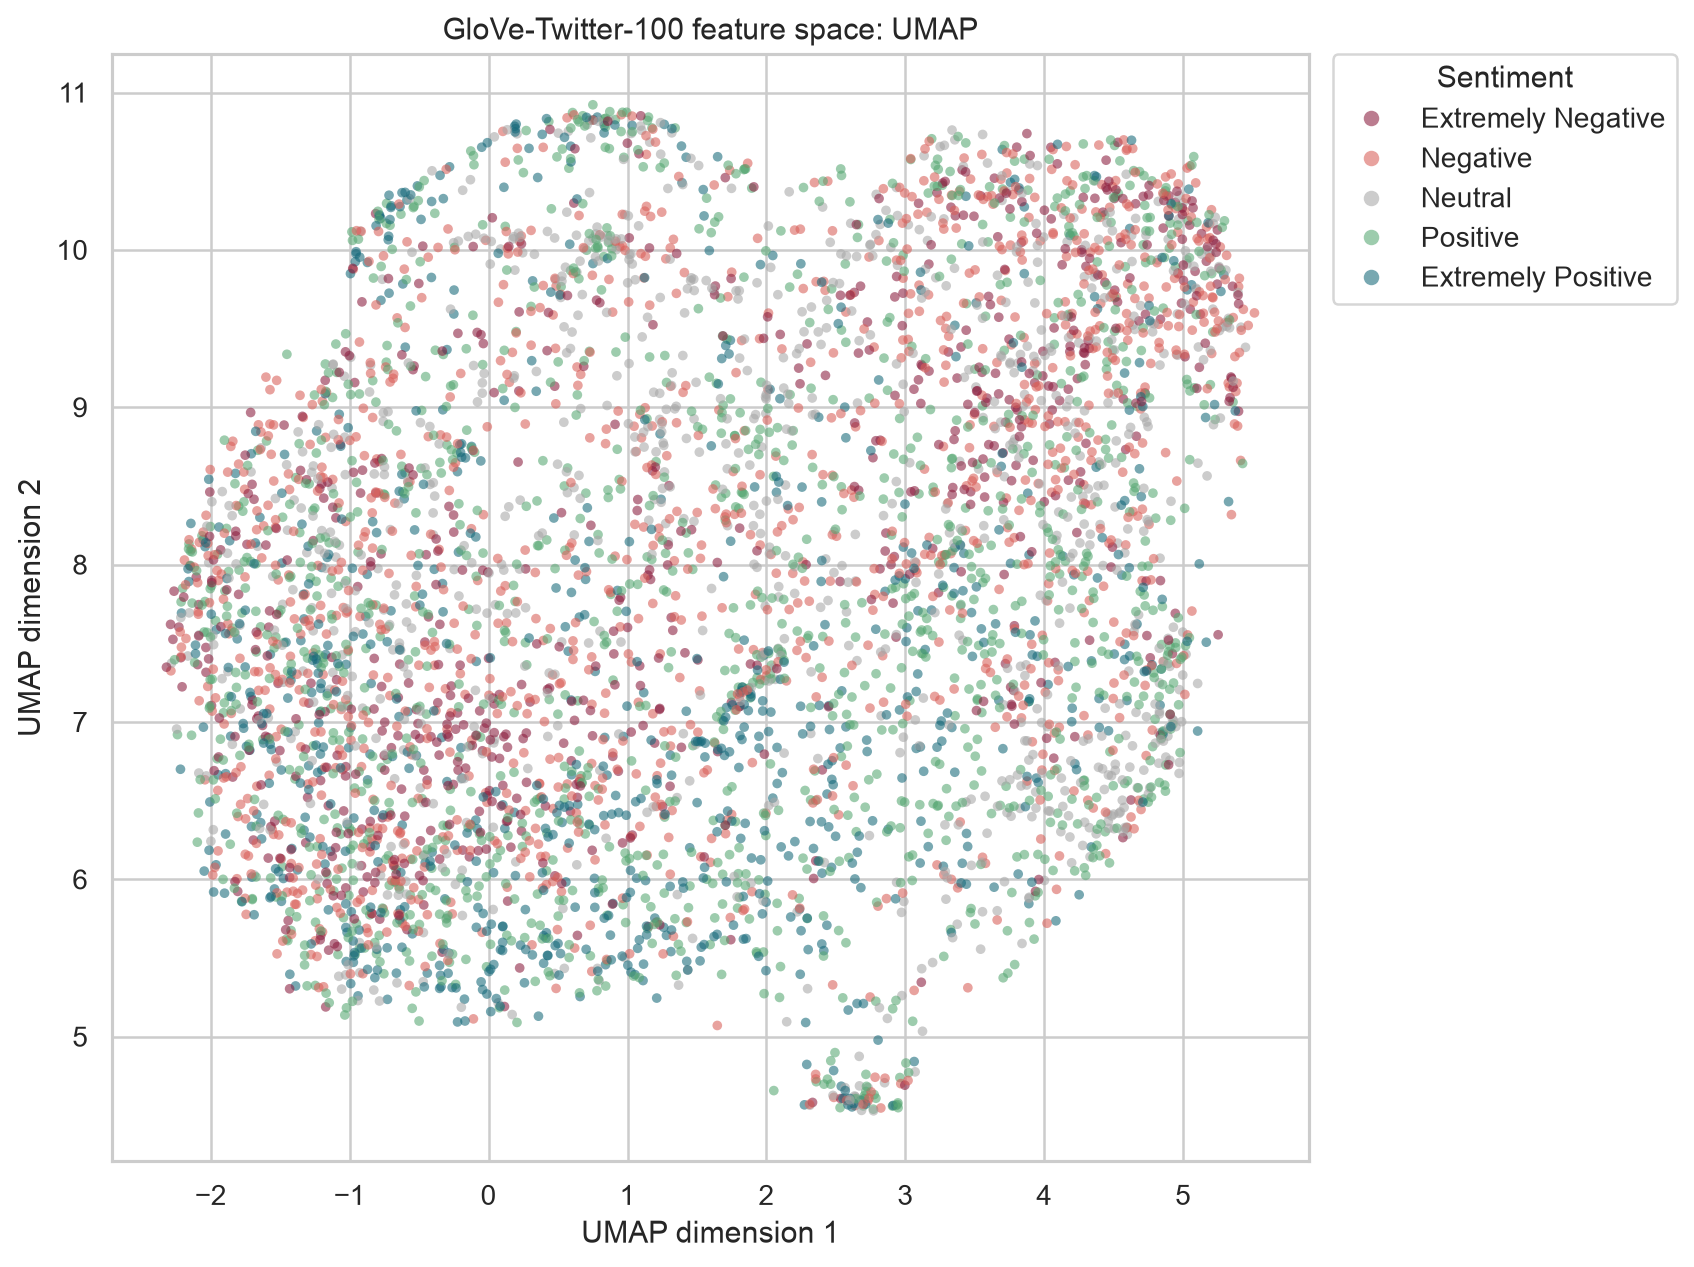
\includegraphics[width=0.49\textwidth]{../outputs/graphics/feature_space/glove/umap.png}
\caption{UMAP projections of TF-IDF (left) and GloVe (right), using cosine distance on their respective 50-dimensional PCA/SVD representations.}
\label{fig:feature-umap}
\end{figure}

All six projections show considerable colour overlap, so neither representation forms five 
naturally isolated sentiment clusters. TF-IDF's nonlinear views contain several local islands, 
but most islands mix labels and may reflect shared vocabulary or topics rather than sentiment 
alone. GloVe shows broad local sentiment tendencies in places, yet adjacent and extreme 
classes still overlap heavily. The visual overlap anticipates the neighbouring-class errors 
discussed in Section~\ref{sec:analysis}, but it is not a substitute for evaluation. 